\section{Versuchsaufbau und Durchführung}
\subsection{Aufgabe 1: Darstellung des Messsystems}
\subsection{Aufgabe 2: MVC Durchführung}
\subsection{Aufgabe 3: Darstellung der Ergebnisse aus Aufgabe 2}
\subsection{Aufgabe 4: Aufbau des MVC-Versuchsaufbaus}

Wie in Abbildung \ref{fig:measuring_electrodes} und \ref{fig:GND_electrode_c7} dargestellt, besteht der 
MVC-Versuchsaufbau aus mehreren Komponenten. Am Probanden wurden drei Elektroden angebracht, vergleichbar 
zu jenen, die bereits im Lab~2 verwendet wurden. Zwei Messelektroden wurden auf dem Bauch des Musculus 
biceps brachii platziert, wobei eine Elektrode etwa zwei Zentimeter distal in Richtung der Sehne angebracht 
wurde \ref{fig:measuring_electrodes}. Eine Referenz- bzw. Groundelektrode wurde auf dem Dornfortsatz 
des siebten Halswirbels (C7) positioniert \ref{fig:GND_electrode_c7}. Diese Platzierung wurde gewählt,
um Störungen und bewegungsbedingte Artefakte möglichst gering zu halten.

\begin{figure}[h]
    \centering
    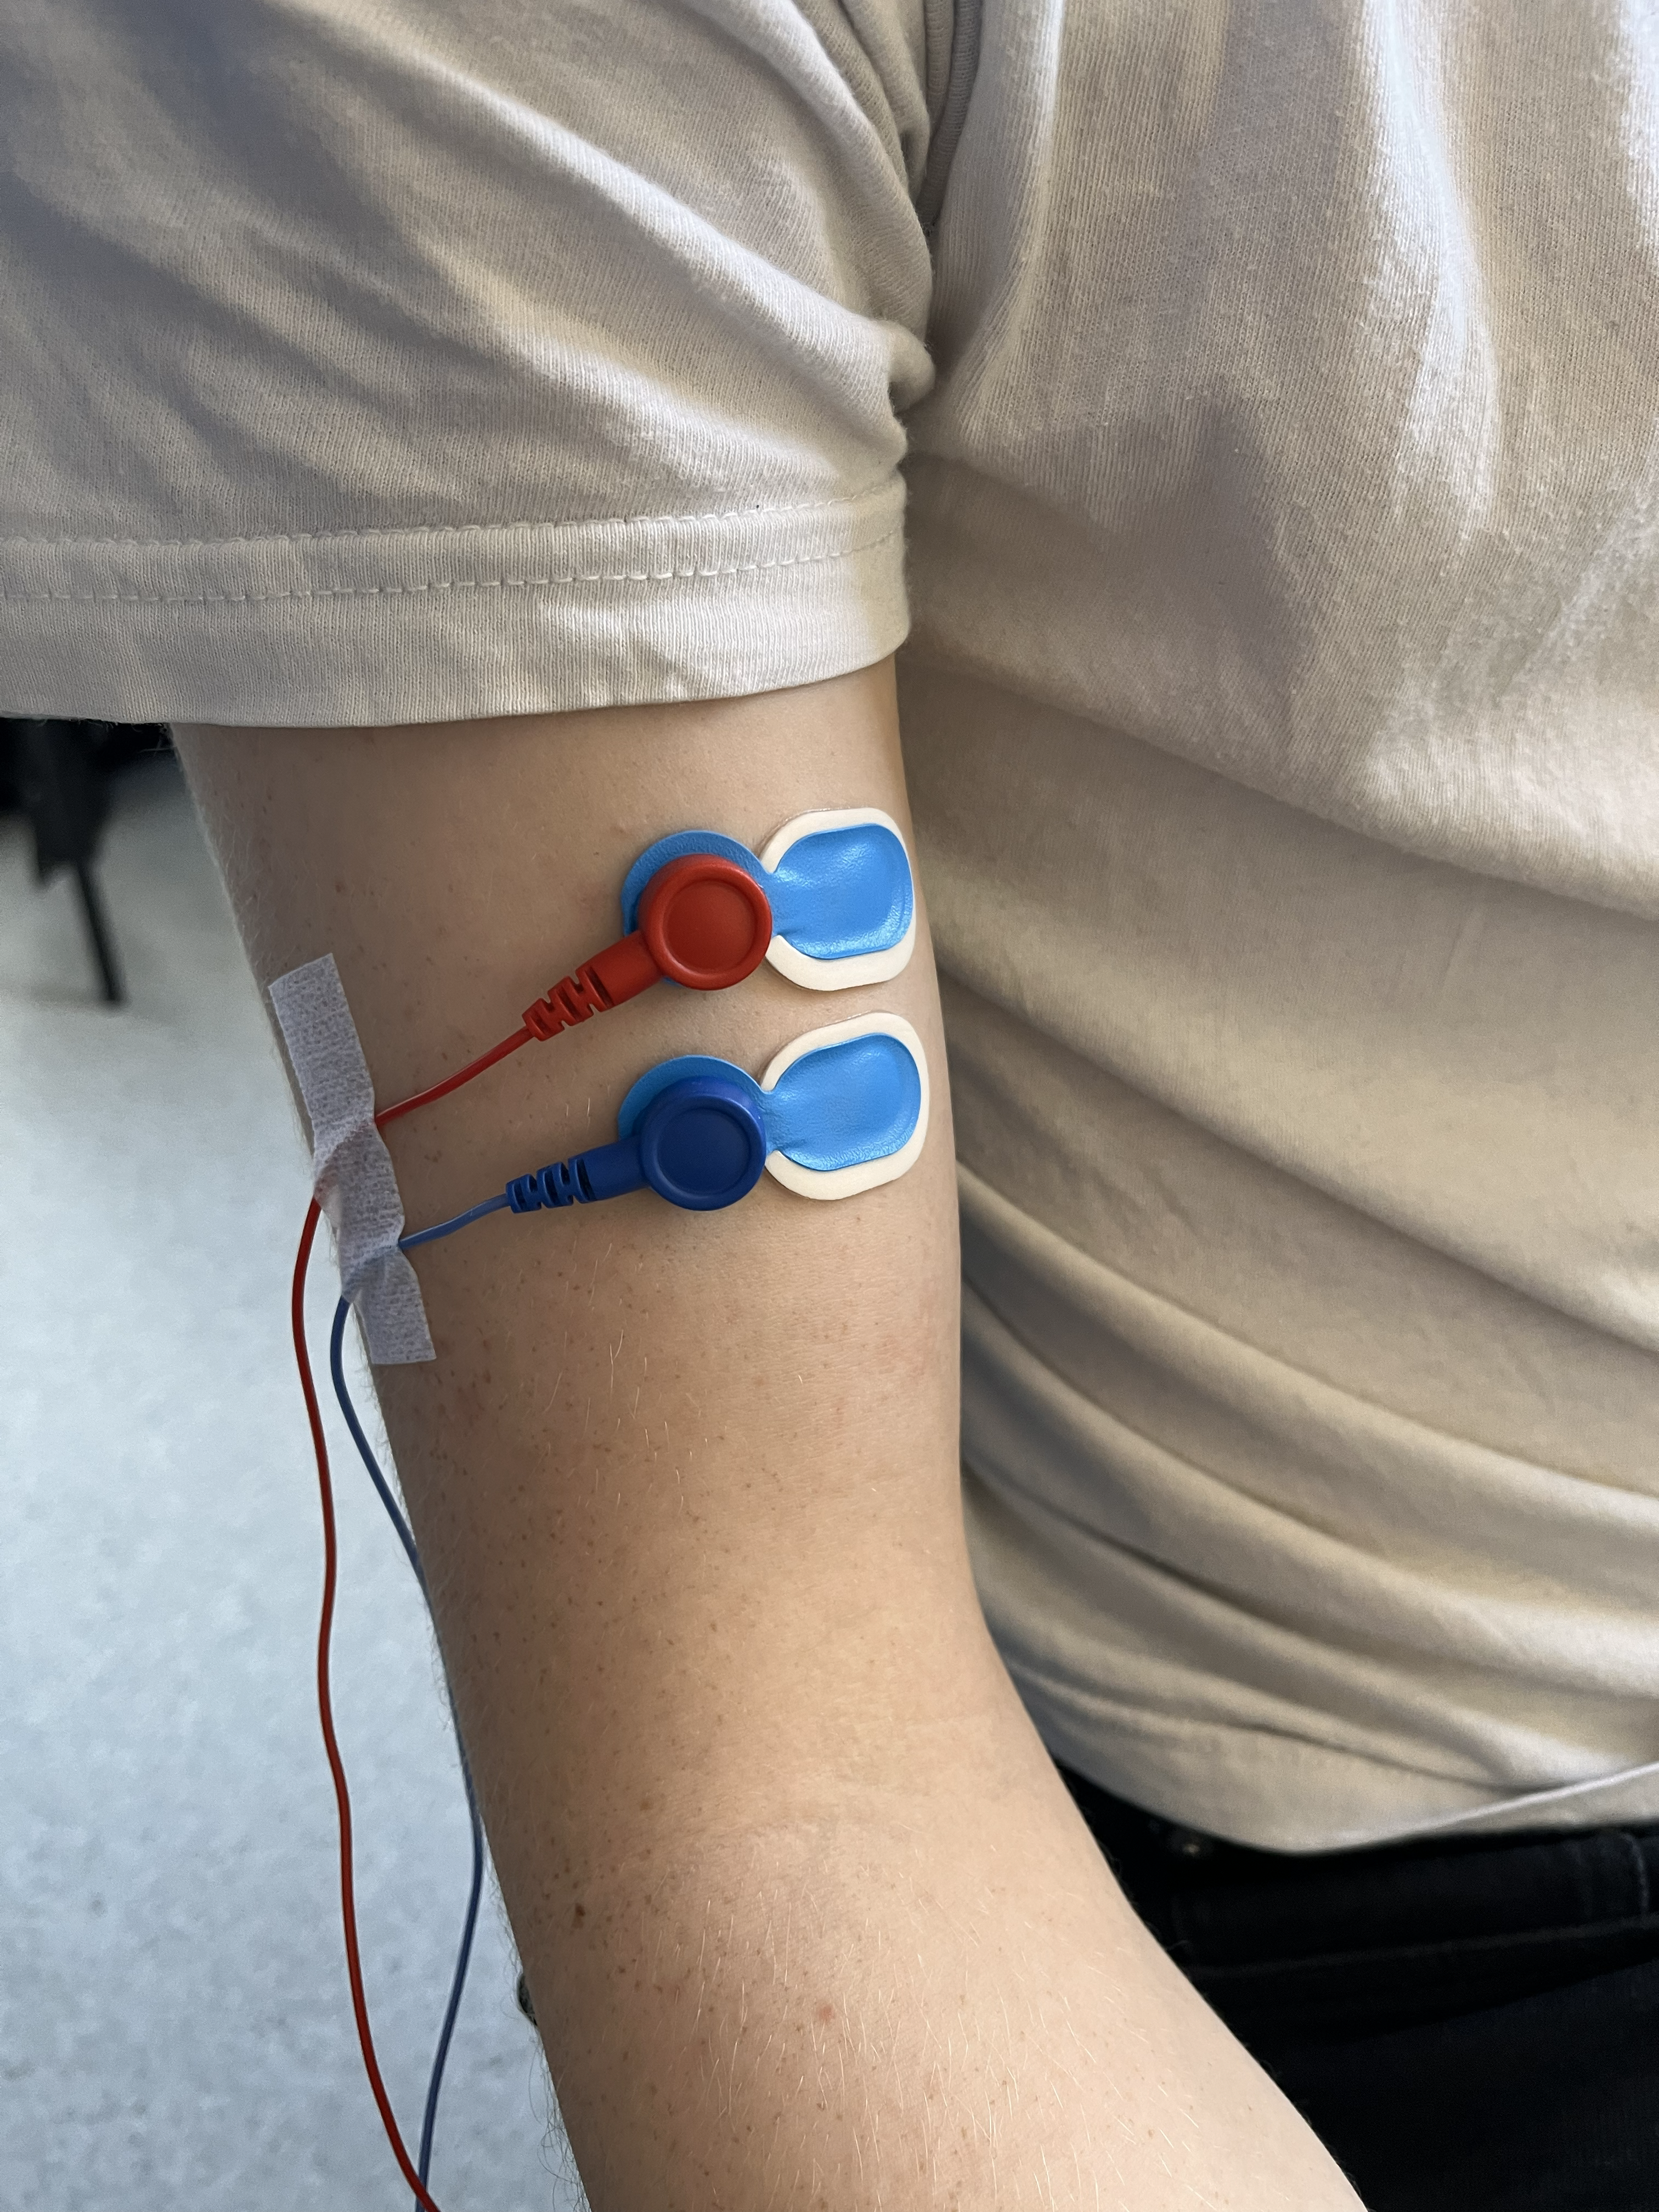
\includegraphics[width=0.3\textwidth]{figures/measuring_electrodes.png}
    \caption{Platzierung der Messelektroden für den MVC-Versuch}
    \label{fig:measuring_electrodes}
\end{figure}

\begin{figure}[h]
    \centering
    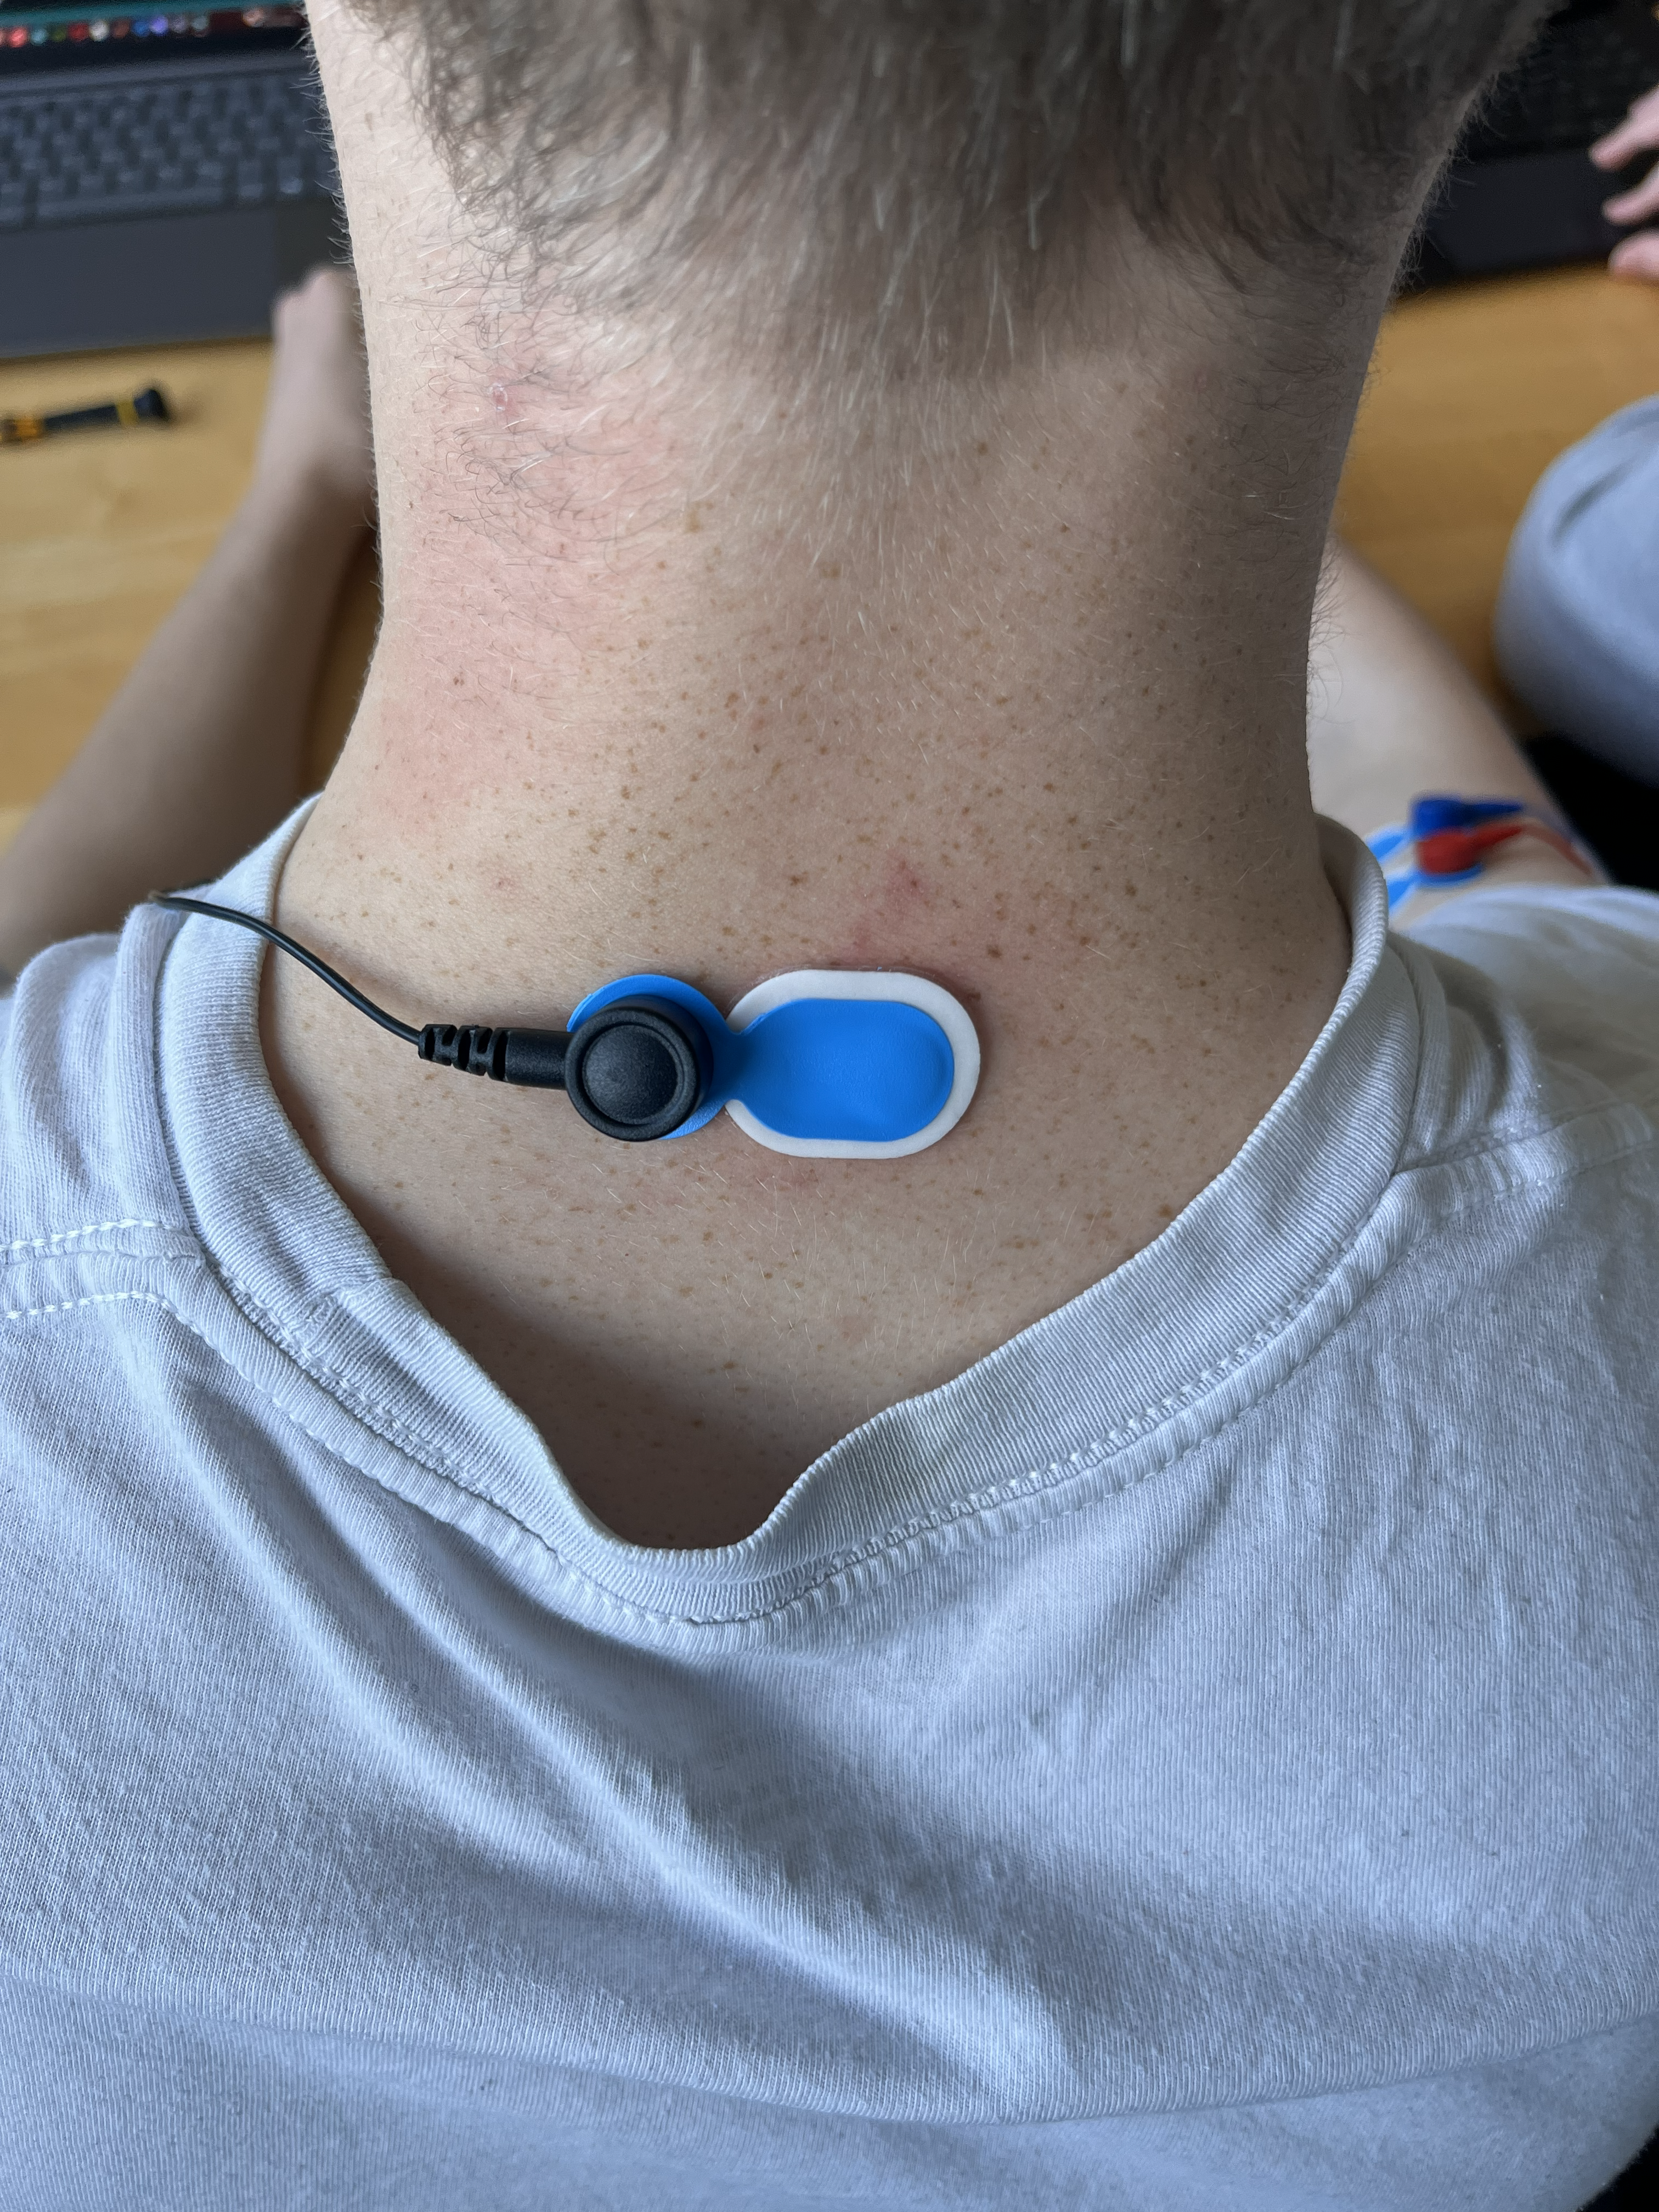
\includegraphics[width=0.3\textwidth]{figures/GND_electrode_c7.png}
    \caption{Platzierung der GND-Elektrode auf dem C7-Wirbel}
    \label{fig:GND_electrode_c7}
\end{figure}

Wie in Abbildung \ref{fig:biceps_tension} zu erkennen ist, sitzt der Proband auf einem Stuhl, wobei der 
Unterarm auf dem Oberschenkel aufliegt. Dadurch stellt sich mit minimaler Bewegung ein etwa 90°-Winkel 
zwischen Ober- und Unterarm ein. Das Handgelenk liegt an der Unterkante des Tisches an. Zur Bestimmung der 
maximalen willkürlichen Kontraktion wird der Proband angewiesen, mit maximaler Kraft zu versuchen, den 
Tisch anzuheben. Gleichzeitig sitzt eine weitere Person auf dem Tisch, um sicherzustellen, dass dieser 
unbeweglich bleibt und keine sichtbare Bewegung stattfinden kann.

\begin{figure}[h]
    \centering
    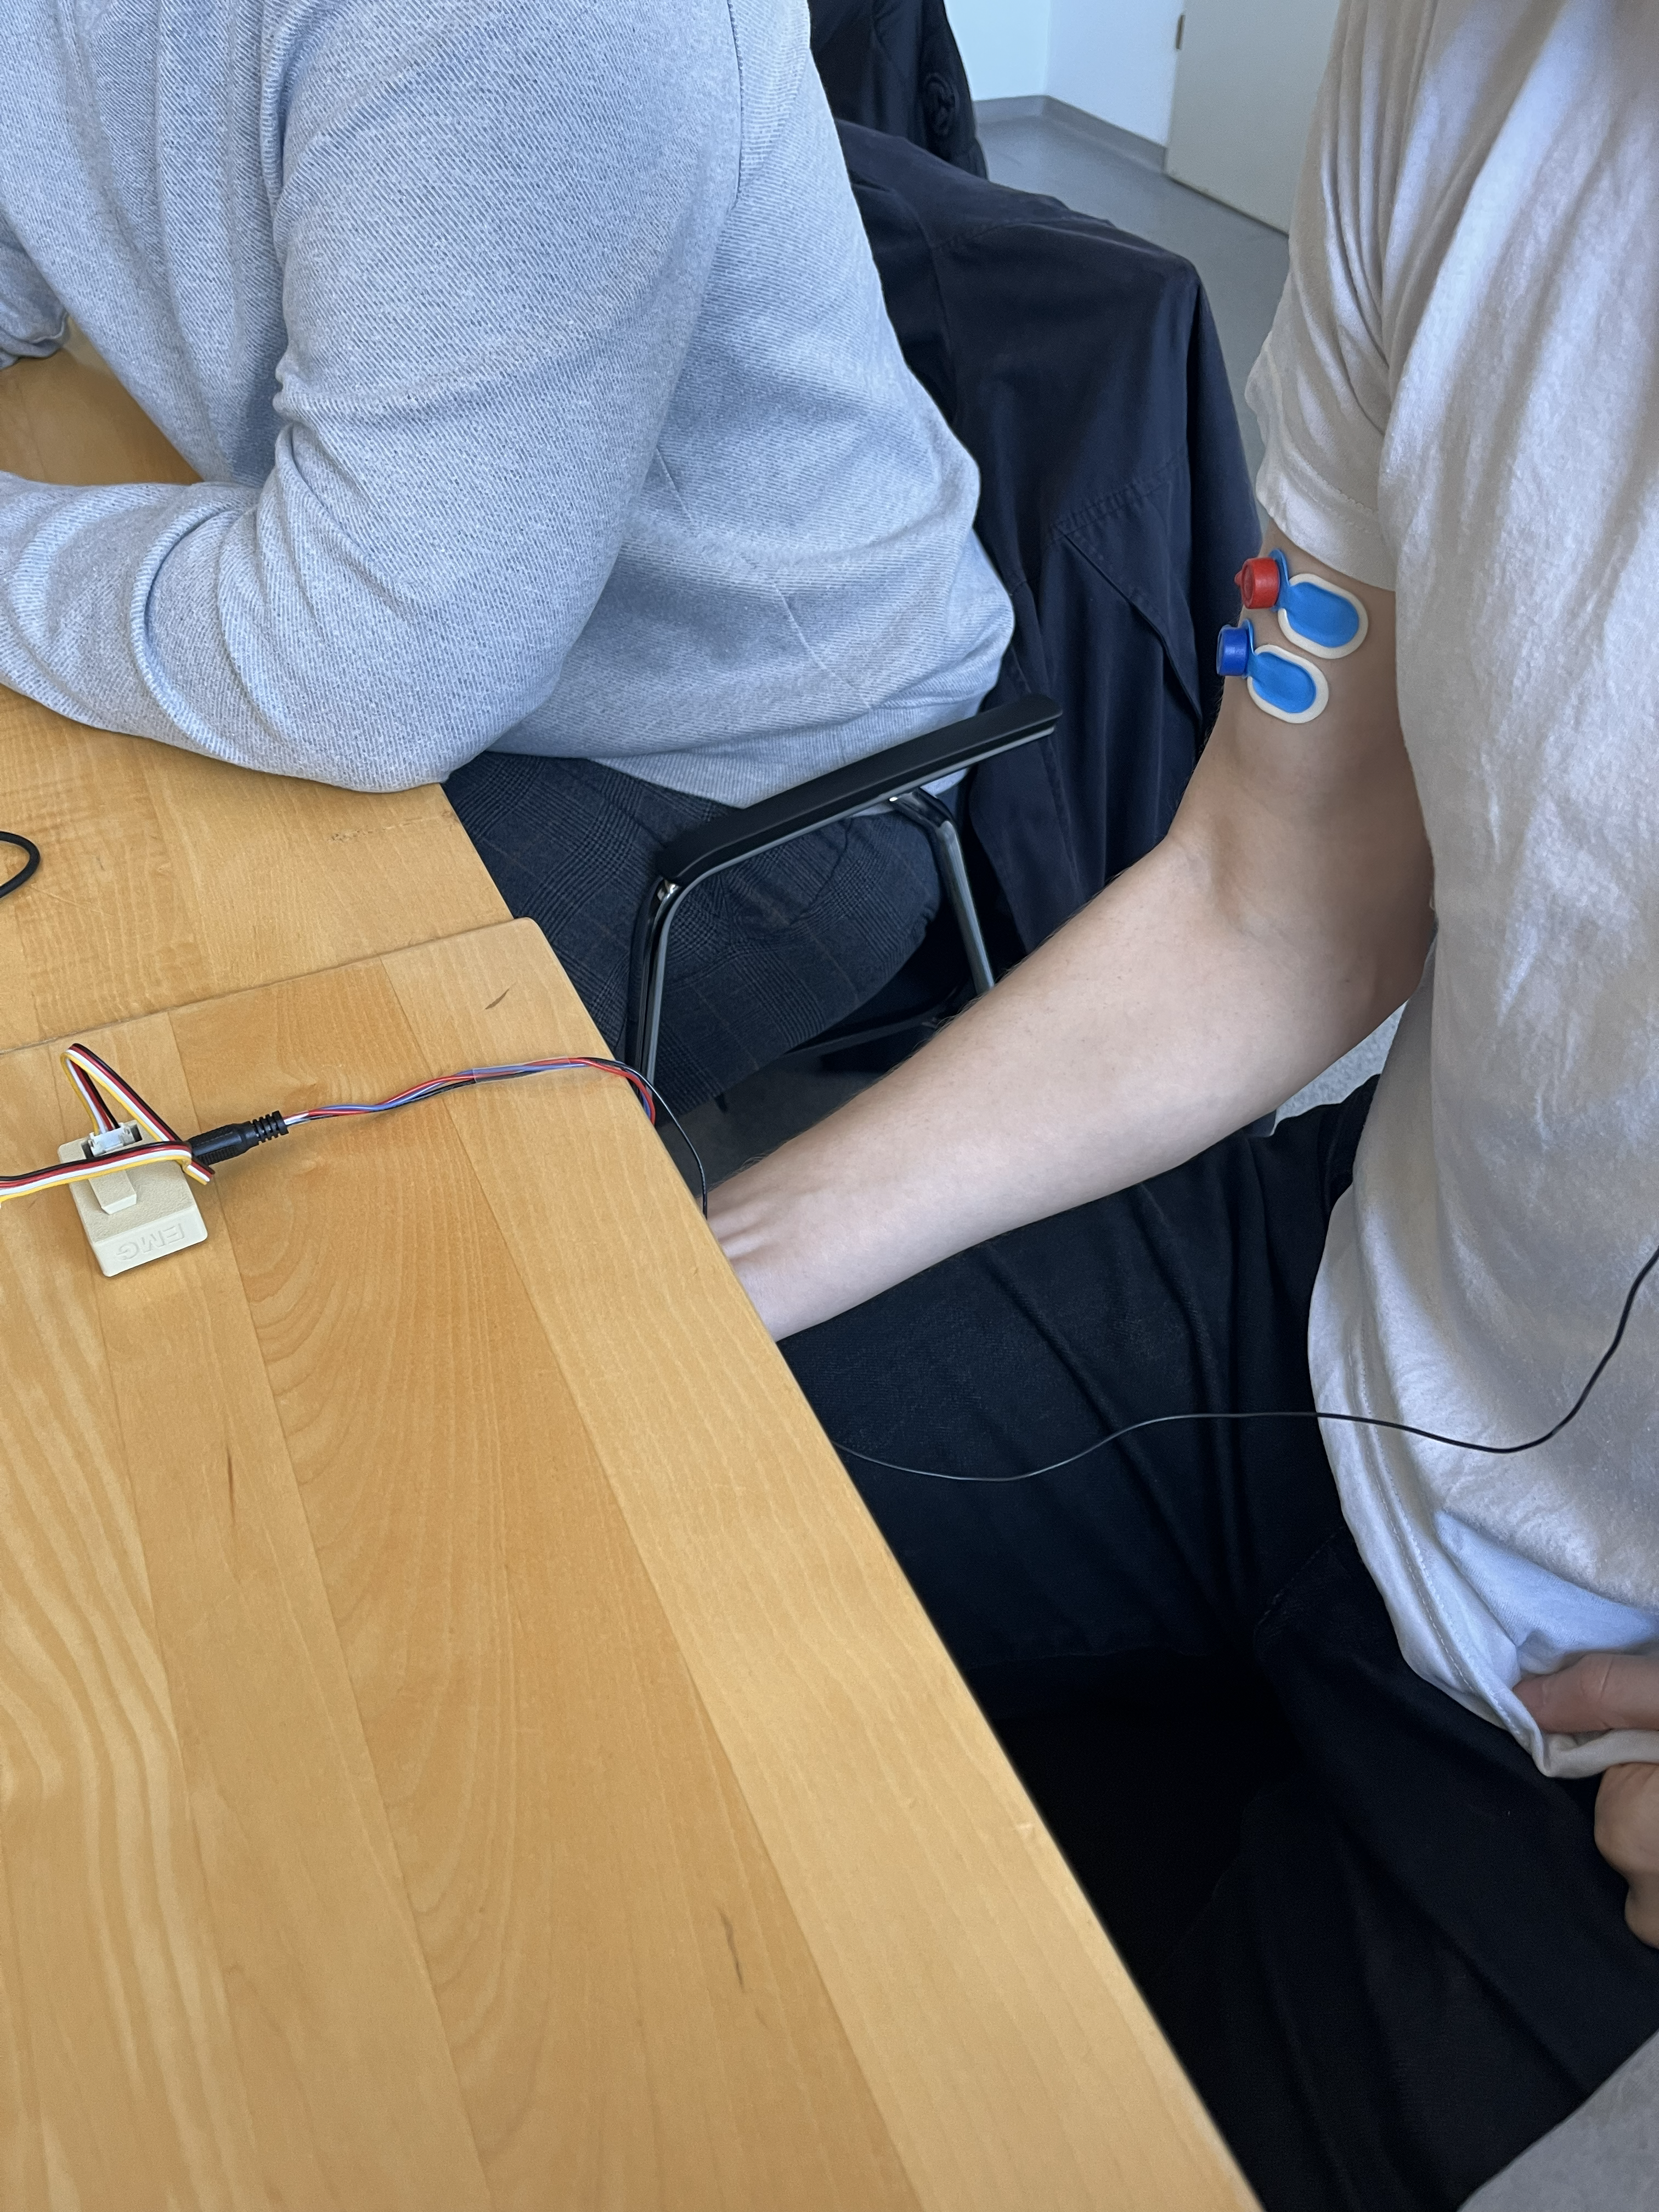
\includegraphics[width=0.4\textwidth]{figures/biceps_tension.png}
    \caption{Angespannter Zustand des Bizeps während des MVC-Versuchs}
    \label{fig:biceps_tension}
\end{figure}

Durch diesen Versuchsaufbau wird eine isometrische Kontraktion des Musculus biceps brachii ermöglicht, 
bei der der Muskel Kraft entwickelt, ohne sich zu verkürzen. Die gewählte Gelenkstellung begünstigt zudem 
eine nahezu optimale Länge-Spannungs-Relation des Muskels. In Kombination mit der stabilen Körperhaltung 
und dem unbeweglichen Widerstand erlaubt dies eine maximale Rekrutierung motorischer Einheiten und somit 
eine maximale willkürliche Kontraktion.

Die maximale Anspannung wird für acht bis zehn Sekunden gehalten, während die EMG-Daten aufgezeichnet 
werden. Dieser Vorgang wird dreimal wiederholt, wobei zwischen den einzelnen Versuchen eine Pause von etwa
einer Minute eingehalten wird, um muskuläre Ermüdung zu vermeiden. Der MVC-Versuch wurde für alle drei 
Gruppenmitglieder durchgeführt.

Der Bizeps Brachii lässt sich in diesem Versuchsaufbau maximal kontrahieren, da sich um eine isometrische 
Kontraktion handelt und dadurch kein Kraftverlust durch Beschleunigung auftritt.
Zudem bedeutet der 90°-Winkel zwischen Ober- und Unterarm, dass der Bizeps in einer optimalen Länge für
die maximale Kraftentwicklung ist.
\subsection{Aufgabe 5: Experiment 2 -Relative Muskelaktivierung}
\subsection{Aufgabe 6: Experiment 3 - Ermüdung}
\subsection{Aufgabe 7: Darstellung des Leistungsspektrums}
Wie in Abbildung \ref{fig:beispielbild} dargestellt, zeigt das Leistungsspektrum des EMG-Signals eine 
deutliche Konzentration der spektralen Anteile im niedrigen Frequenzbereich.

\begin{figure}[h]
    \centering
    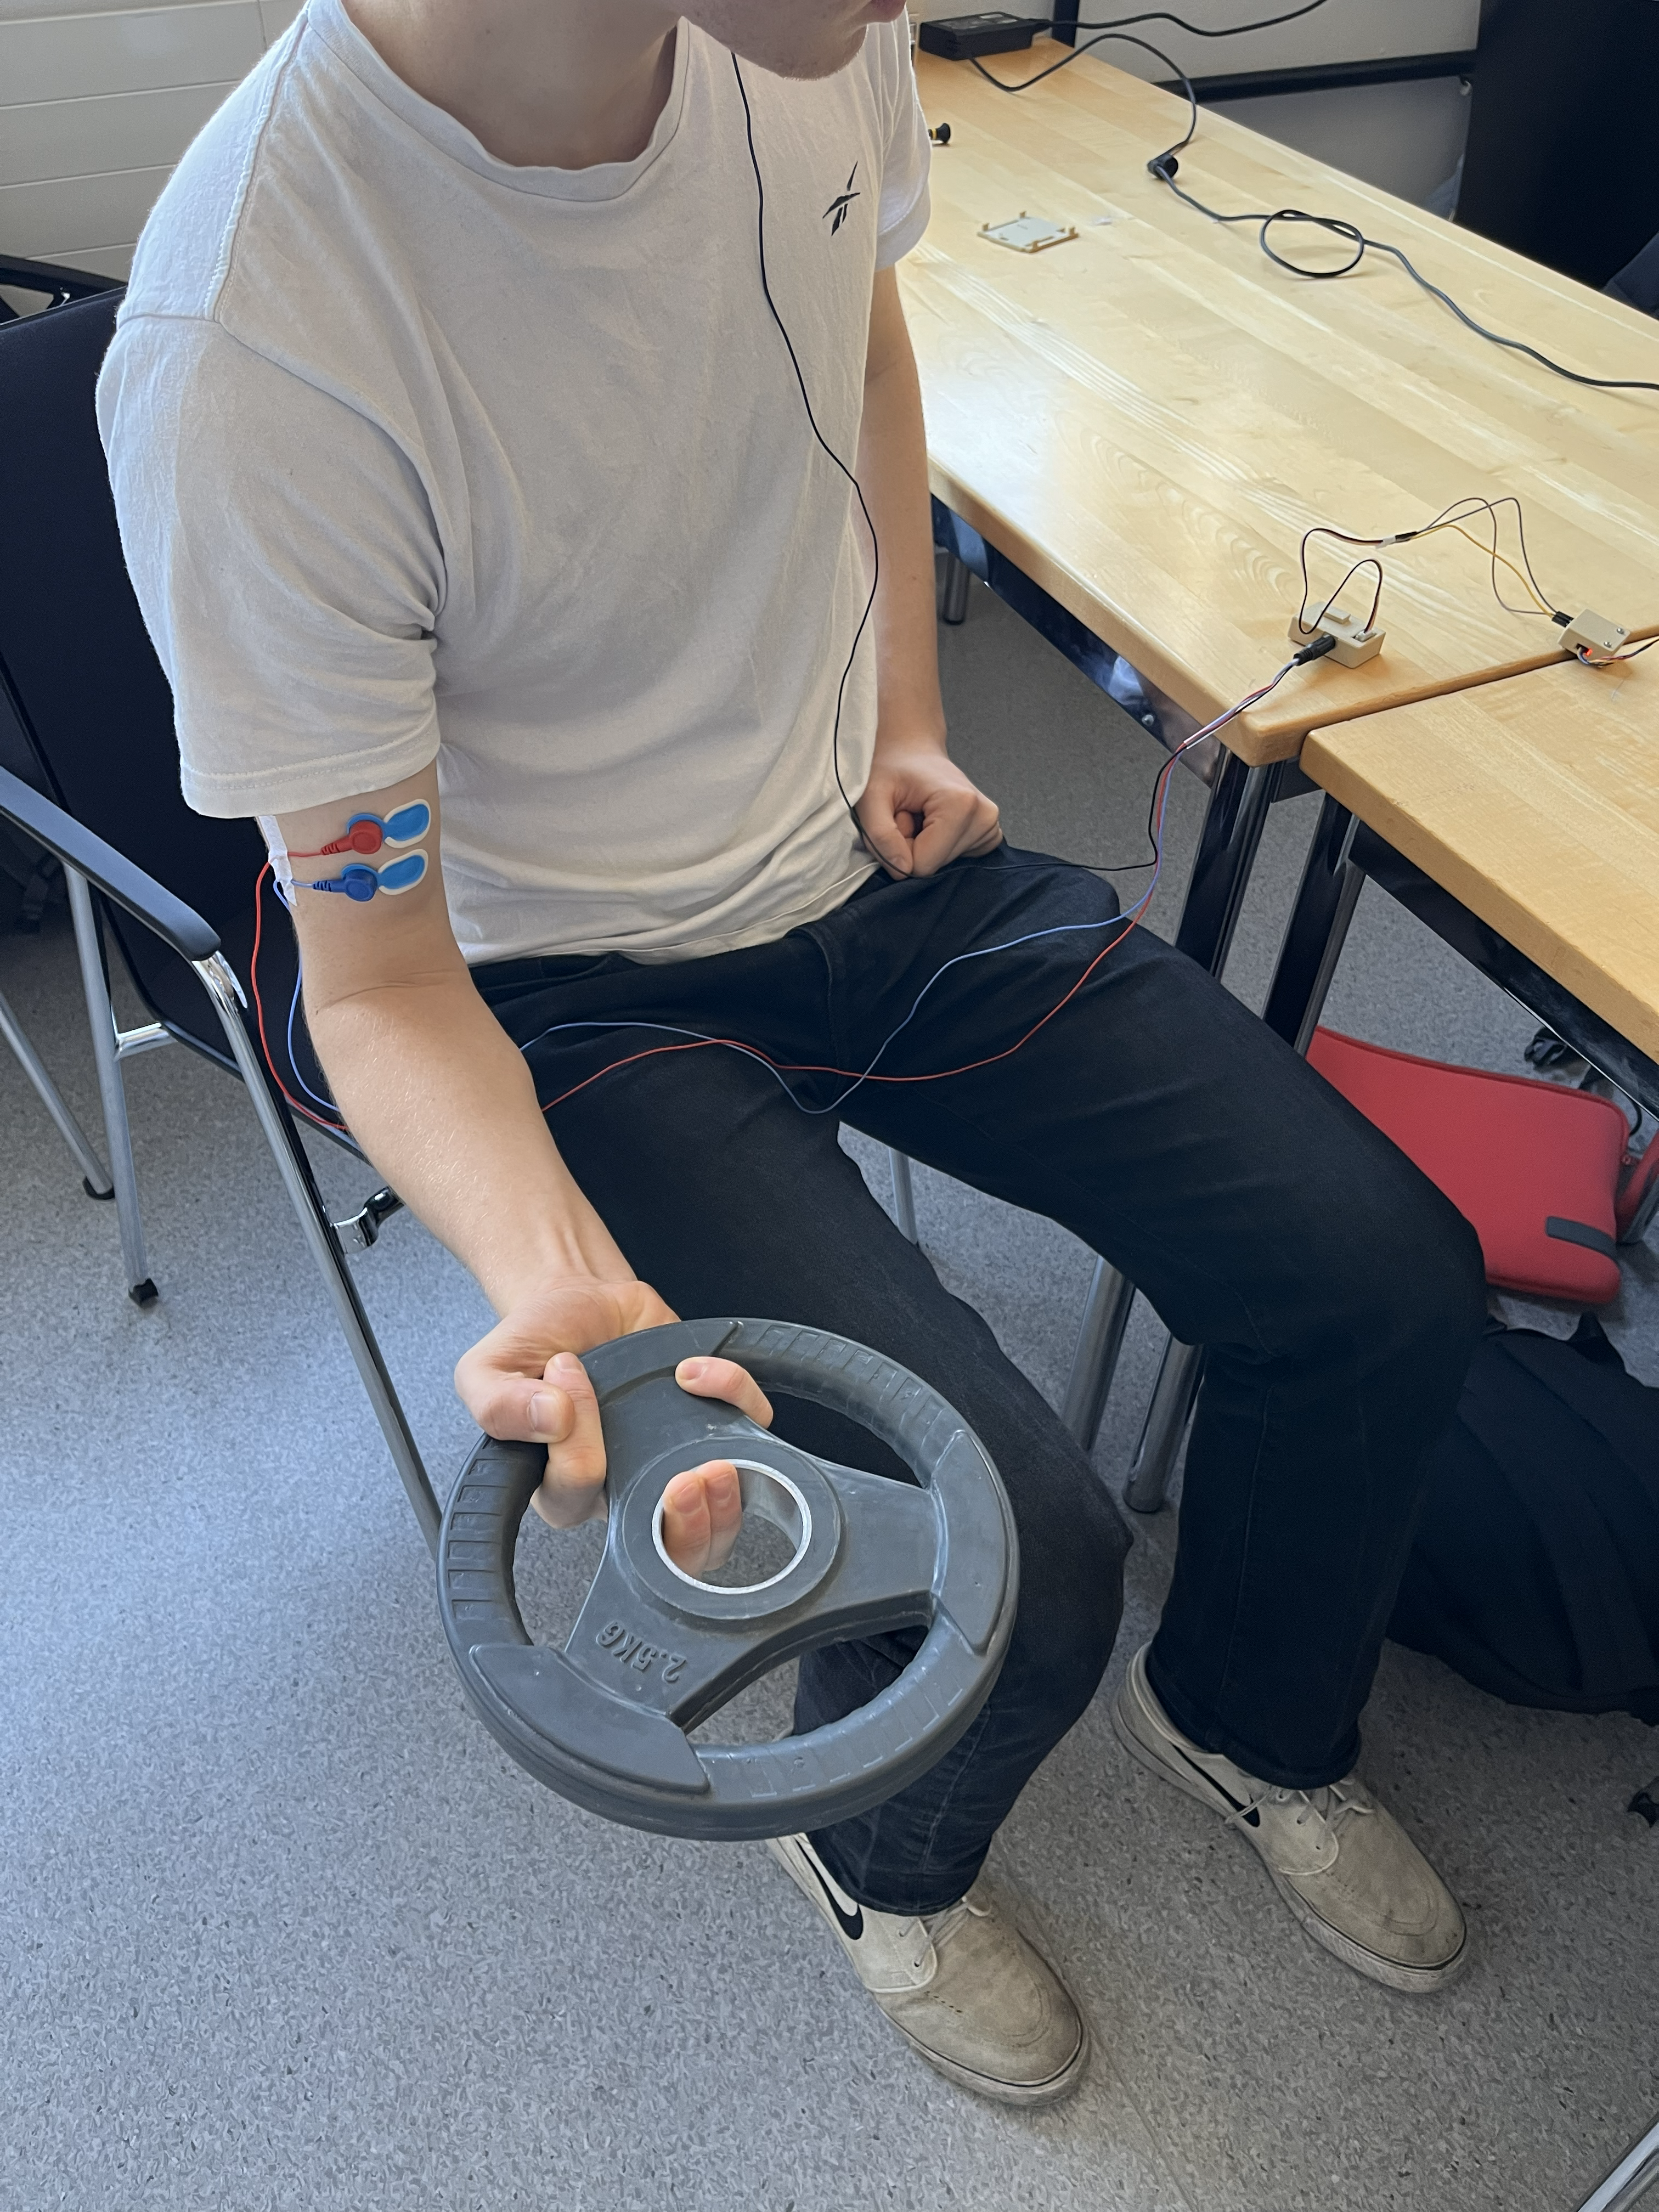
\includegraphics[width=0.3\textwidth]{figures/weight1.png}
    \caption{Beispielhaftes Leistungsspektrum eines EMG-Signals während einer isometrischen Kontraktion}
    \label{fig:beispielbild}
\end{figure}

Dieses Spektralverhalten ist charakteristisch für EMG-Signale während isometrischer Kontraktionen und 
statischer Haltearbeit. Entsprechend liegt auch die Medianfrequenz des Leistungsspektrums im unteren 
Frequenzbereich. Dies weist auf eine dominante Aktivierung von Typ-I-Muskelfasern (Slow-Twitch-Fasern) 
hin, die aufgrund ihrer geringen Kontraktionsgeschwindigkeit und hohen Ermüdungsresistenz besonders für 
ausdauernde Belastungen geeignet sind.

Da das statische Halten eines Gewichts über einen längeren Zeitraum eine Ausdauer- und keine 
Schnellkraftbelastung darstellt, ist die niedrige Medianfrequenz physiologisch plausibel. Veränderungen 
der Medianfrequenz im zeitlichen Verlauf können nach Merletti \cite{Merletti1999SENIAM_SignalProcessing} somit als geeigneter Indikator für muskuläre 
Ermüdungsprozesse herangezogen werden, da eine Abnahme der Medianfrequenz typischerweise mit einer 
Reduktion der Muskelfaserleitgeschwindigkeit einhergeht.

\subsection{Aufgabe 8: Medianfrequenz des Leistungsspektrums}